\documentclass[11pt,a4paper]{article}
\usepackage[margin=1in]{geometry}
\usepackage{graphicx}
\usepackage{booktabs}
\usepackage{float}
\usepackage{wrapfig}
\usepackage[hypertexnames=false]{hyperref}

\title{Optimization of Partitioned Hash Join with Duplicates}
\author{Gianluca Panzani}
\date{\today}
\setcounter{secnumdepth}{3}
\setcounter{tocdepth}{3}

\begin{document}
\begin{titlepage}
    \centering
    {\Large University of Pisa\par}
    \vspace{0.6cm}
    {\large Parallel and Distributed Systems\par}
    \vspace{2.0cm}
    {\LARGE \textbf{Optimization of Partitioned Hash Join with Duplicates}\par}
    \vspace{1.2cm}
    {\large Module 3 - Report\par}
    \vfill
    {\large Gianluca Panzani\par}
    \vspace{0.3cm}
    {\large \today\par}
\end{titlepage}

\pagenumbering{roman}
\tableofcontents
\newpage
\pagenumbering{arabic}


% Implementation
\section{Implementation}


% Executable variants
\subsection{Executable variants}
The repository contains one sequential baseline and six OpenMP executables which are compared each other. There are three kind of OpenMP families based on the type of parallelization strategy: \texttt{loop}, \texttt{task} and \texttt{taskloop}. The last one is added only as an experimental comparison, to see whether OpenMP's taskloop construct behaves closer to manual tasks or to ordinary loop scheduling. Each family also has a \texttt{\_wb} version that adds workload balancing on the join phase. All versions use the same flat open-addressing count table in the local build/probe phase, so the comparison is mostly about the parallel execution model and scheduling policy, not about a different join algorithm. So at the end we have the following six executables: \texttt{hashjoin\_seq}, \texttt{hashjoin\_omp\_loop}, \texttt{hashjoin\_omp\_loop\_wb}, \texttt{hashjoin\_omp\_task}, \texttt{hashjoin\_omp\_task\_wb}, \texttt{hashjoin\_omp\_taskloop} and \texttt{hashjoin\_omp\_taskloop\_wb}.

% Workflow
\subsection{Workflow}
The implementation workflow strategy is the following:
\begin{itemize}
    \item implement the OpenMP variants,
    \item run correctness checks,
    \item execute an initial larger grid search for each OpenMP family with a uniform dataset,
    \item analyze the generated CSV files with the statistics notebooks,
    \item reduce the grid to the most promising parameter regions,
    \item run the reduced campaign on uniform and skewed datasets to analyze how the different parallelization strategies perform on the different datasets.
\end{itemize}

% Parameters
\subsection{Parameters}
The benchmark scripts run Slurm jobs on one node of the \texttt{spmcluster} and append one CSV row per configuration in \texttt{src/results/}. The fixed parameters of the main campaign are \(N_R=N_S=50\,000\,000\), \(P=256\), \texttt{seed=13}, \texttt{max\_key=1\,000\,000} and block size \(32768\) in the reduced grid.

The parameters of the final grids were not chosen directly. Initially i've created a larger grid for each family type and then, analyzing the relative notebook files, i've chosen the most promising values because of the huge amount of combinations. The grid of the \texttt{loop} family explores OpenMP schedules (\texttt{static}, \texttt{dynamic}, \texttt{guided}), chunk sizes, partition/join thread counts and partition block sizes. The grid of the \texttt{task} one explores the number of input blocks per partition task, the number of partitions per join task, offset-task granularity and thread counts. And the grid of the experimental \texttt{taskloop} family explores the same decomposition through \texttt{taskloop} grainsizes.

The reduced grid used for the final results keeps the most stable choices found by those statistics files: guided scheduling for loop variants, explicit task grains in the range 2--4 for the task variants, taskloop grains in the range 2--8 for the experimental taskloop variants, 32 join threads for each family, and 32 or 64 partition threads.

Three datasets are measured. The uniform dataset is the same pseudo-random generation scheme used in the previous module. The skewed datasets are generated with the format \texttt{skewed\_R\_H} with: \(R\%\) percentage of records sampled from keys that map to the first \(H\%\) of partitions. In the final grids i've used \texttt{skewed\_90\_5} and \texttt{skewed\_90\_1}, which concentrate 90\% of the records respectively into about 13 and 3 hot partitions.


% Parallelization Strategy
\section{Parallelization Strategy}

% Partition phase
\subsection{Partition phase}
In the loop versions, the available work is exposed as regular OpenMP loops and the runtime scheduling policy decides how iterations are assigned to threads. This keeps the code compact and makes schedule tuning simple: the same executable can test \texttt{static}, \texttt{dynamic} and \texttt{guided} behavior through \texttt{schedule(runtime)}. In practice this strategy is well suited when the work units are regular and numerous, because the OpenMP loop scheduler has low overhead and the tuning space is mostly reduced to schedule, chunk size and thread count.

The task versions use a more explicit decomposition. Instead of relying only on loop iteration scheduling, they create OpenMP tasks over groups of blocks and partition ranges. This gives more control over the granularity of the work submitted to the runtime, but it also introduces a more delicate tradeoff: small tasks improve balancing opportunities but increase task creation overhead, while large tasks reduce overhead but behave closer to coarse loop chunks. For this reason the task grid includes task-grain parameters in addition to the thread counts.

The taskloop version preserves the loop-shaped formulation but asks OpenMP to generate tasks from it, using \texttt{taskloop grainsize(...)}. It is simpler than manually creating explicit tasks and, in the results, often behaves competitively; however, the comparison on which we are focusing on remains between the sequential version and the loop/task strategies.

% Join phase
\subsection{Join phase}
After partitioning, the join phase is naturally parallel because partition \(p\) of \(R\) only has to be joined with partition \(p\) of \(S\). In other words, for each pair of partitions the join is independent.

The loop versions express this with an OpenMP \texttt{for} loop over the partition ids and combine the final \texttt{join\_count}, \texttt{checksum1} and \texttt{checksum2} with an OpenMP \texttt{reduction}. The task versions instead create explicit OpenMP \texttt{task}s for groups of partition joins and each task writes its result into a private \texttt{partial} slot (while the global result is computed after \texttt{taskwait}).

The important distinction is between the non-\texttt{\_wb} and the \texttt{\_wb} executables. In the non-\texttt{\_wb} versions, the join work is submitted to OpenMP in the natural partition-id order \(0,\ldots,P-1\). This is simple and works well when the dataset is uniform, because partitions have similar sizes and each local join has roughly similar cost.

With skewed datasets, however, some partitions contain many more records and duplicate matches. Then a raw partition-id order can create a tail effect: most threads finish their small partitions while some few threads remain busy on hot partitions. The \texttt{\_wb} variants address this by keeping the same local hash-join code and the same final reduction, but changing the work list given to OpenMP. Before the join starts, partitions are sorted by estimated work,
\[
    |R_p| + |S_p|,
\]
from largest to smallest. The loop \texttt{\_wb} version uses \texttt{schedule(dynamic,1)} on this ordered list, so threads repeatedly take the next heaviest remaining partition. The task \texttt{\_wb} version creates tasks over the ordered list instead of over raw partition ids. It exposes expensive partitions earlier and reduces tail imbalance. It still cannot split one single hot partition across multiple threads, which is why the performances are limited with skewed datasets.

\begin{figure}[H]
    \centering
    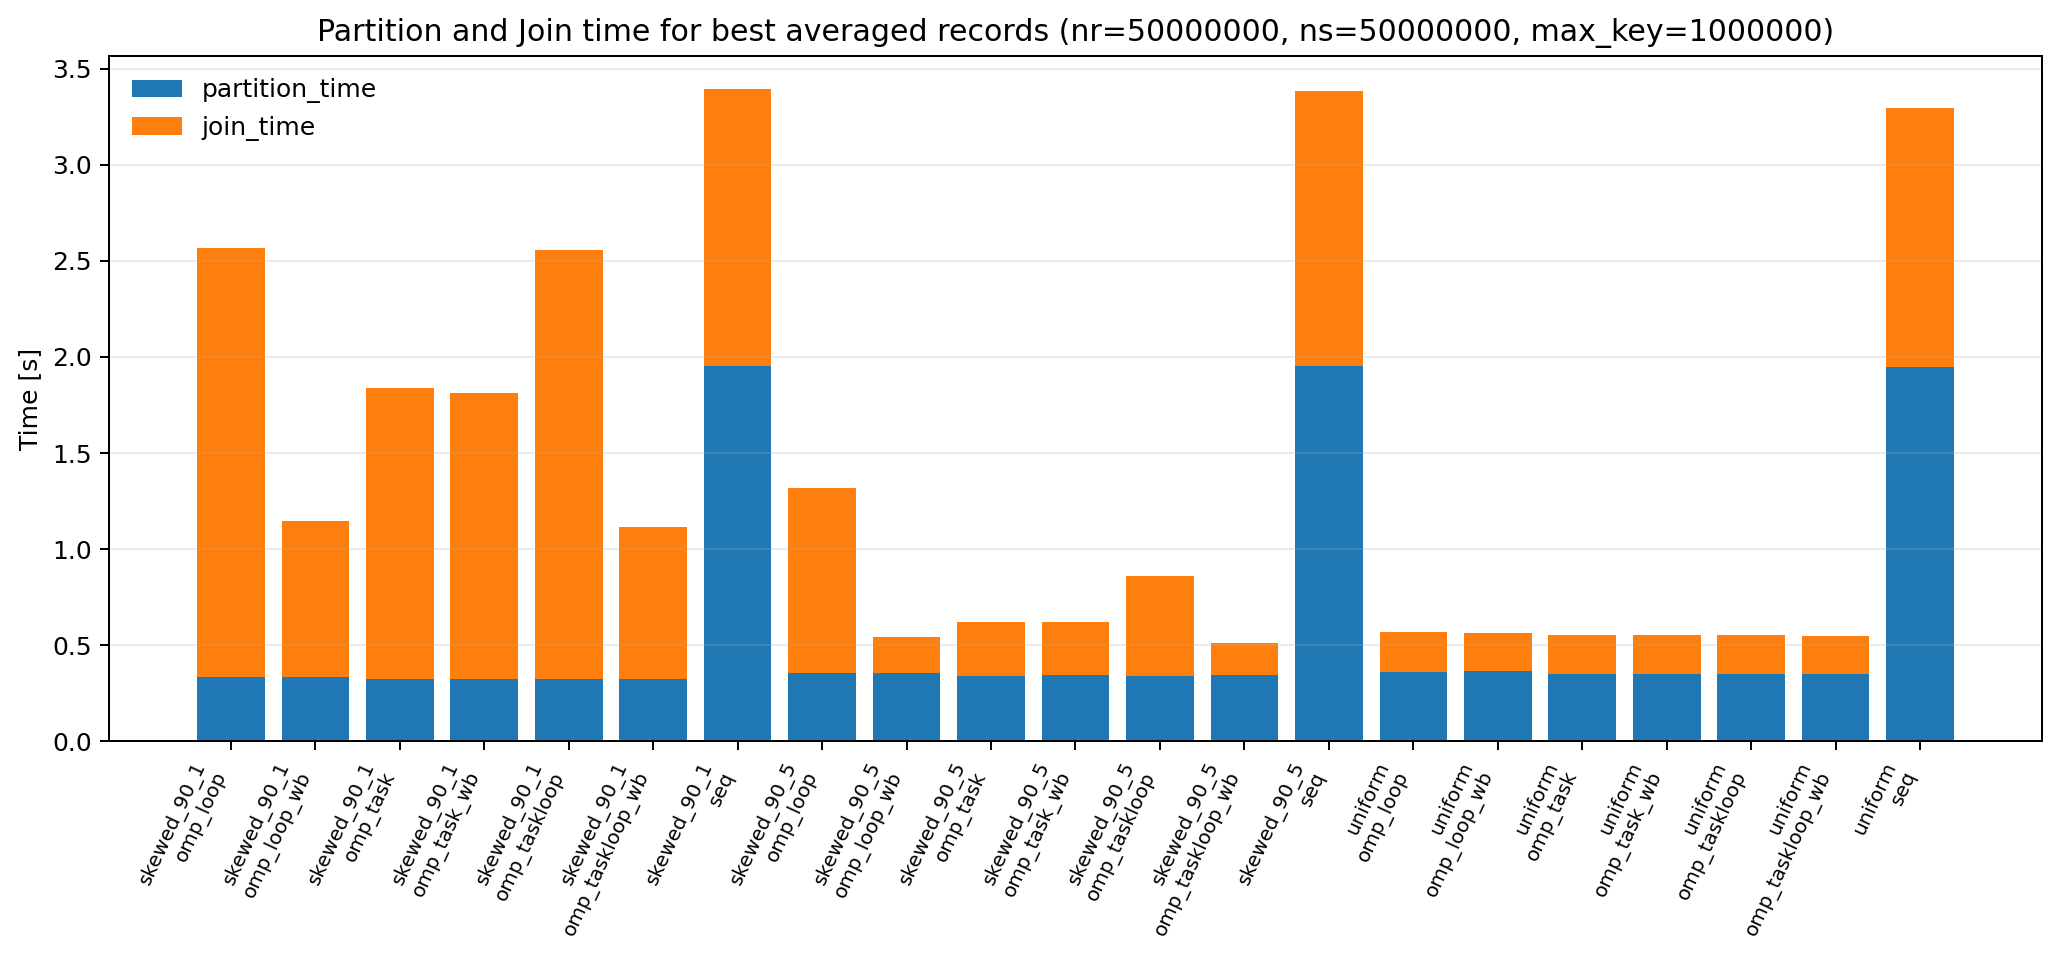
\includegraphics[width=0.82\linewidth]{../img/005_selected_best_phase_breakdown_50000000_50000000_1000000.png}
    \caption{Comparison between partition and join times for each dataset type and executables combination.}
    \label{fig:partition-join-time}
\end{figure}


% Results Analysis
\section{Results Analysis}
All results below are generated from \texttt{src/results/}. The best sequential times in the current campaign are \(3.114\) s for the uniform dataset, \(3.258\) s for \texttt{skewed\_90\_5}, and \(3.256\) s for \texttt{skewed\_90\_1}. The best Module 2 C++ threaded result available in \texttt{src/old\_results/} was \(0.507\) s for \texttt{hashjoin\_par\_pj\_wb\_map}; the best broad-grid OpenMP result here is \(0.539\) s, so the final OpenMP implementation is close in absolute time but does not clearly improve over the previous C++ threaded best case. This covers the main Module 3 comparison: sequential baseline, OpenMP loop, OpenMP tasks, the extra taskloop experiment, uniform/skewed workloads, and the previous C++ threaded implementation.

\begin{figure}[H]
    \centering
    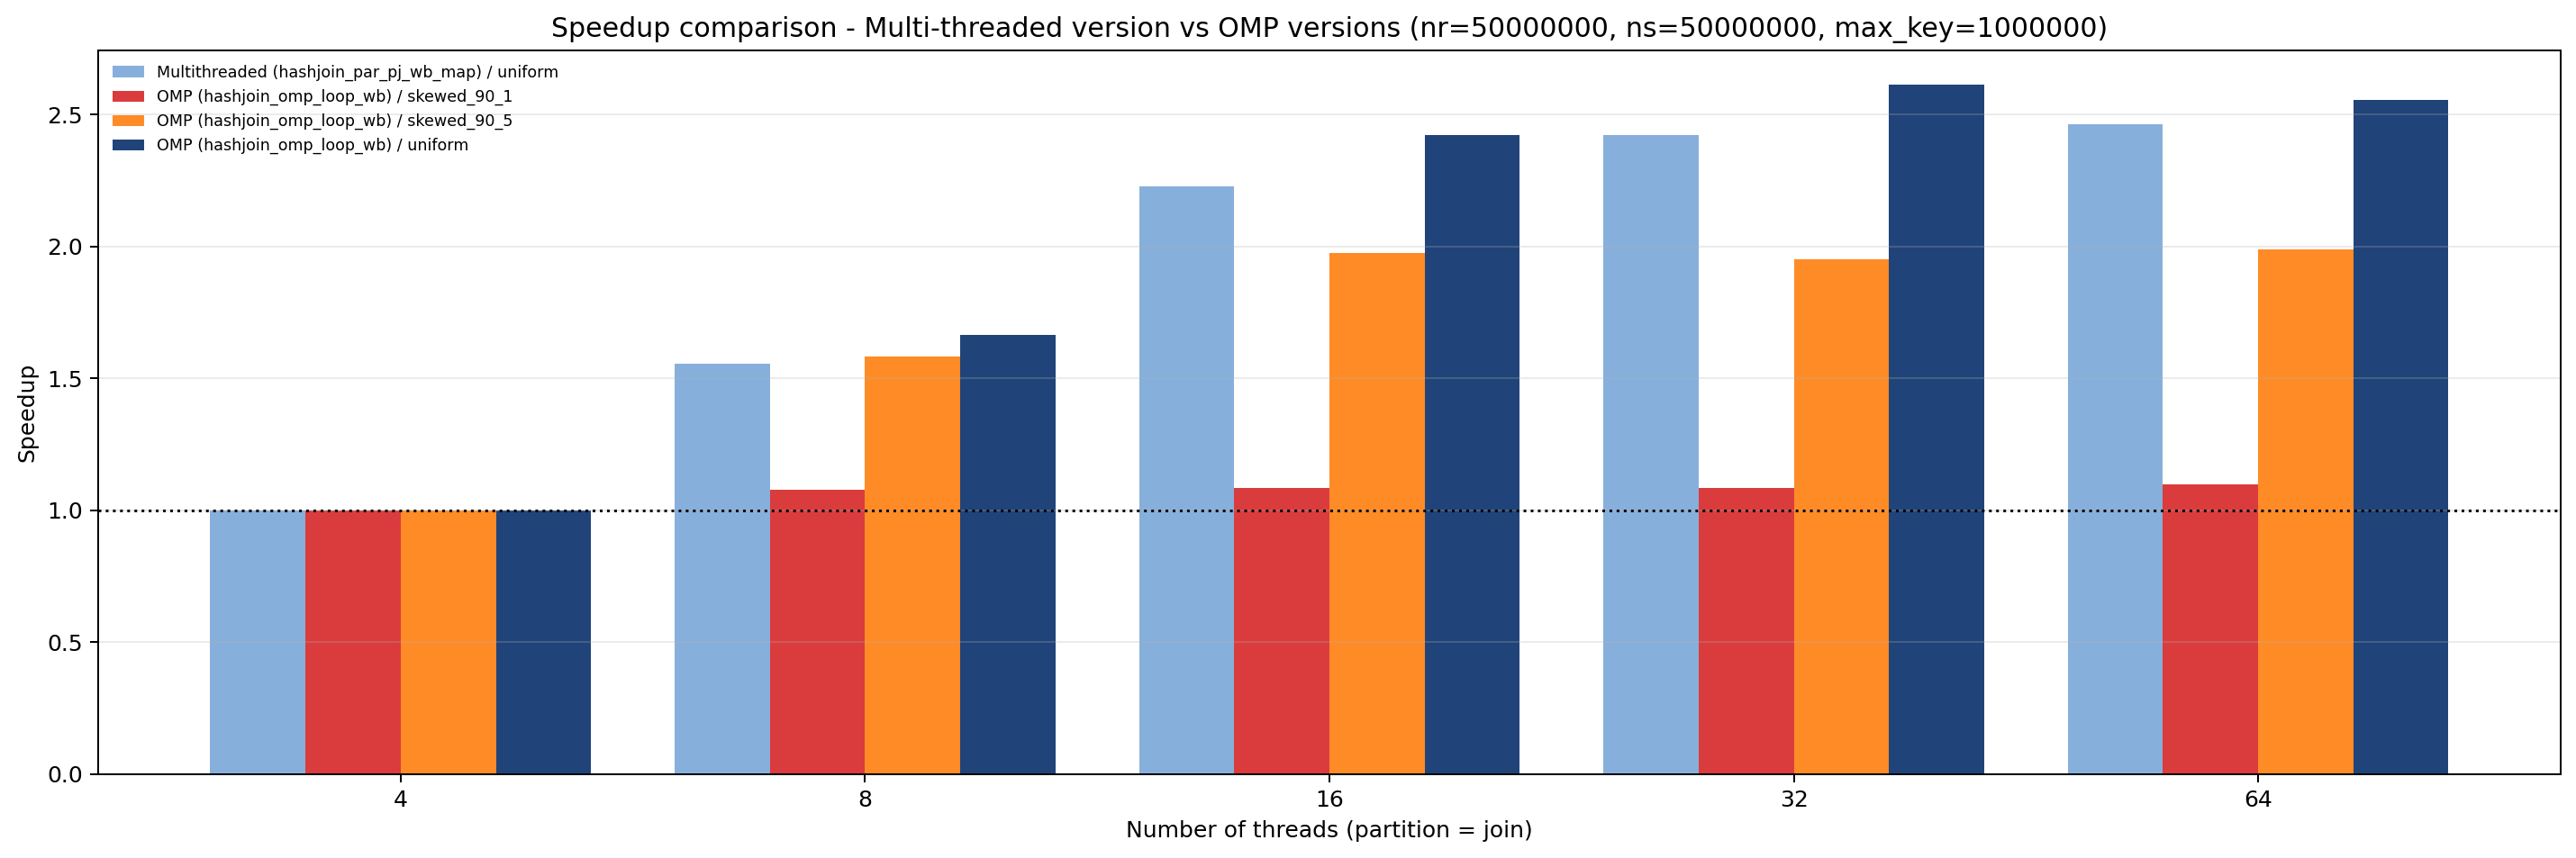
\includegraphics[width=0.86\linewidth]{../img/007_strong_scaling_speedup_50000000_50000000_1000000.png}
    \caption{Speedup comparison between the previous multi-threaded \texttt{hashjoin\_par\_pj\_wb\_map} executable and the selected OpenMP workload-balanced loop implementation.}
    \label{fig:module2-vs-omp-speedup}
\end{figure}


% Uniform dataset
\subsection{Uniform dataset}
On the uniform workload, all complete OpenMP implementations are close once both partition and join are parallelized. The best time is obtained by \texttt{hashjoin\_omp\_taskloop\_wb} with 64 partition threads and 32 join threads: \(0.539\) s, corresponding to \(5.78\times\) speedup over the current sequential baseline.

\begin{table}[H]
    \centering
    \small
    \begin{tabular}{lrrrr}
        \toprule
        Variant & \(T_{part}\) & \(T_{join}\) & Best time [s] & Speedup \\
        \midrule
        \texttt{omp\_loop} & 32 & 32 & 0.568 & \(5.49\times\) \\
        \texttt{omp\_loop\_wb} & 32 & 32 & 0.561 & \(5.55\times\) \\
        \texttt{omp\_task} & 64 & 32 & 0.545 & \(5.72\times\) \\
        \texttt{omp\_task\_wb} & 64 & 32 & 0.542 & \(5.74\times\) \\
        \texttt{omp\_taskloop} & 64 & 32 & 0.544 & \(5.73\times\) \\
        \texttt{omp\_taskloop\_wb} & 64 & 32 & 0.539 & \(5.78\times\) \\
        \bottomrule
    \end{tabular}
    \caption{Best observed uniform-dataset configuration per OpenMP executable.}
    \label{tab:uniform-best}
\end{table}

The difference between the best loop, task and taskloop versions is small; this means that, for uniform partitions, OpenMP tasking does not add much by itself. The dominant gains come from parallelizing the join and from keeping the local hash table cache-friendly.
Inside the required implementations, explicit tasks are slightly faster than loop scheduling on uniform data: \texttt{omp\_task} reaches \(0.545\) s against \(0.568\) s for \texttt{omp\_loop}, and the \texttt{\_wb} pair has the same small gap. The extra taskloop variant is marginally the best overall in this dataset and is also simpler to express than manual task creation, because OpenMP handles the task generation from the loop structure.
The \texttt{taskloop} rows are reported only for experimental comparison: the assignment-required comparison is between loop-level OpenMP and explicit tasks.

\begin{figure}[H]
    \centering
    \includegraphics[width=0.82\linewidth]{../img/004_selected_best_Speedup_vs_sequential_version_50000000_50000000_1000000.png}
    \caption{Best speedup against the sequential baseline for the current OpenMP campaign.}
    \label{fig:selected-best}
\end{figure}


% Skewed datasets
\subsection{Skewed datasets}
The skewed datasets change both load balance and the actual join workload. The final match count rises from about \(2.50 \cdot 10^9\) on uniform data to \(4.06 \cdot 10^{10}\) on \texttt{skewed\_90\_5} and \(1.74 \cdot 10^{11}\) on \texttt{skewed\_90\_1}. Therefore the slowdown is not only scheduling overhead: the hot partitions also contain many more duplicate matches.

\begin{table}[H]
    \centering
    \scriptsize
    \begin{tabular}{llrrrrr}
        \toprule
        Dataset & Variant & \(T_{part}\) & \(T_{join}\) & Best time [s] & Join time [s] & Speedup \\
        \midrule
        \texttt{skewed\_90\_5} & \texttt{omp\_loop} & 32 & 32 & 1.281 & 0.924 & \(2.54\times\) \\
        \texttt{skewed\_90\_5} & \texttt{omp\_loop\_wb} & 32 & 32 & 0.525 & 0.172 & \(6.20\times\) \\
        \texttt{skewed\_90\_5} & \texttt{omp\_task} & 64 & 32 & 0.614 & 0.277 & \(5.31\times\) \\
        \texttt{skewed\_90\_5} & \texttt{omp\_task\_wb} & 64 & 32 & 0.614 & 0.278 & \(5.30\times\) \\
        \texttt{skewed\_90\_5} & \texttt{omp\_taskloop} & 64 & 32 & 0.840 & 0.501 & \(3.88\times\) \\
        \texttt{skewed\_90\_5} & \texttt{omp\_taskloop\_wb} & 64 & 32 & 0.501 & 0.163 & \(6.51\times\) \\
        \midrule
        \texttt{skewed\_90\_1} & \texttt{omp\_loop} & 32 & 32 & 2.558 & 2.222 & \(1.27\times\) \\
        \texttt{skewed\_90\_1} & \texttt{omp\_loop\_wb} & 32 & 32 & 1.120 & 0.783 & \(2.91\times\) \\
        \texttt{skewed\_90\_1} & \texttt{omp\_task} & 64 & 32 & 1.802 & 1.484 & \(1.81\times\) \\
        \texttt{skewed\_90\_1} & \texttt{omp\_task\_wb} & 64 & 32 & 1.799 & 1.480 & \(1.81\times\) \\
        \texttt{skewed\_90\_1} & \texttt{omp\_taskloop} & 64 & 32 & 2.539 & 2.222 & \(1.28\times\) \\
        \texttt{skewed\_90\_1} & \texttt{omp\_taskloop\_wb} & 64 & 32 & 1.101 & 0.781 & \(2.96\times\) \\
        \bottomrule
    \end{tabular}
    \caption{Best observed skewed-dataset result for each OpenMP executable, using the corresponding sequential baseline.}
    \label{tab:skewed-best}
\end{table}

The workload-balanced versions are essential under skew. For \texttt{skewed\_90\_5}, the loop version improves from \(1.281\) s to \(0.525\) s when workload balancing is enabled. For \texttt{skewed\_90\_1}, the same change improves from \(2.558\) s to \(1.120\) s. The strongest skew still remains slower because a very small number of partitions becomes too large to be split further by the current partition-level join strategy.

The comparison between the required OpenMP families changes with skew. Loop scheduling performs better than explicit tasks on the skewed datasets once the join work list is balanced: \texttt{omp\_loop\_wb} reaches \(0.525\) s and \(1.120\) s, while \texttt{omp\_task\_wb} remains at \(0.614\) s and \(1.799\) s. The extra taskloop implementation is still useful experimentally: with workload balancing it gives the best skewed times, while keeping the implementation closer to the loop version than to the more verbose explicit-task code.


% Scaling analysis
\section{Scaling analysis}
Strong and weak scalability are measured only with the selected workload-balanced loop implementation, using fixed best parameters from the reduced grid. These plots should therefore be read as scalability of the chosen OpenMP loop solution, not as another comparison among loop, task and taskloop implementations. The loop version is used because it is the selected required implementation for the fixed-parameter scaling drivers; the taskloop version is excluded because it is only an additional experimental comparison.

The \texttt{strong\_scaling.cpp} and \texttt{weak\_scaling.cpp} files are dedicated scaling drivers. Both keep the same algorithm and the same workload-balanced join scheduling used in the final loop executable: guided partition scheduling, workload-ordered dynamic join scheduling, and fixed block/chunk parameters selected from the reduced grid. The strong-scaling driver fixes \(N_R=N_S=50\,000\,000\) and varies the thread count. The weak-scaling driver increases the input from 10M to 80M records per relation while increasing the thread count from 4 to 32.


% Weak scalability
\subsection{Weak scalability}
Weak scaling is moderate. Uniform data keeps the best scaled speedup, reaching about \(2.20\times\) at 32 threads relative to the 4-thread base point, but efficiency still drops to about \(0.28\). The \texttt{skewed\_90\_1} curve is much worse and reaches only \(0.89\times\) scaled speedup at 32 threads, because the enlarged hot partitions increase both imbalance and duplicate-match work.

\begin{figure}[H]
    \centering
    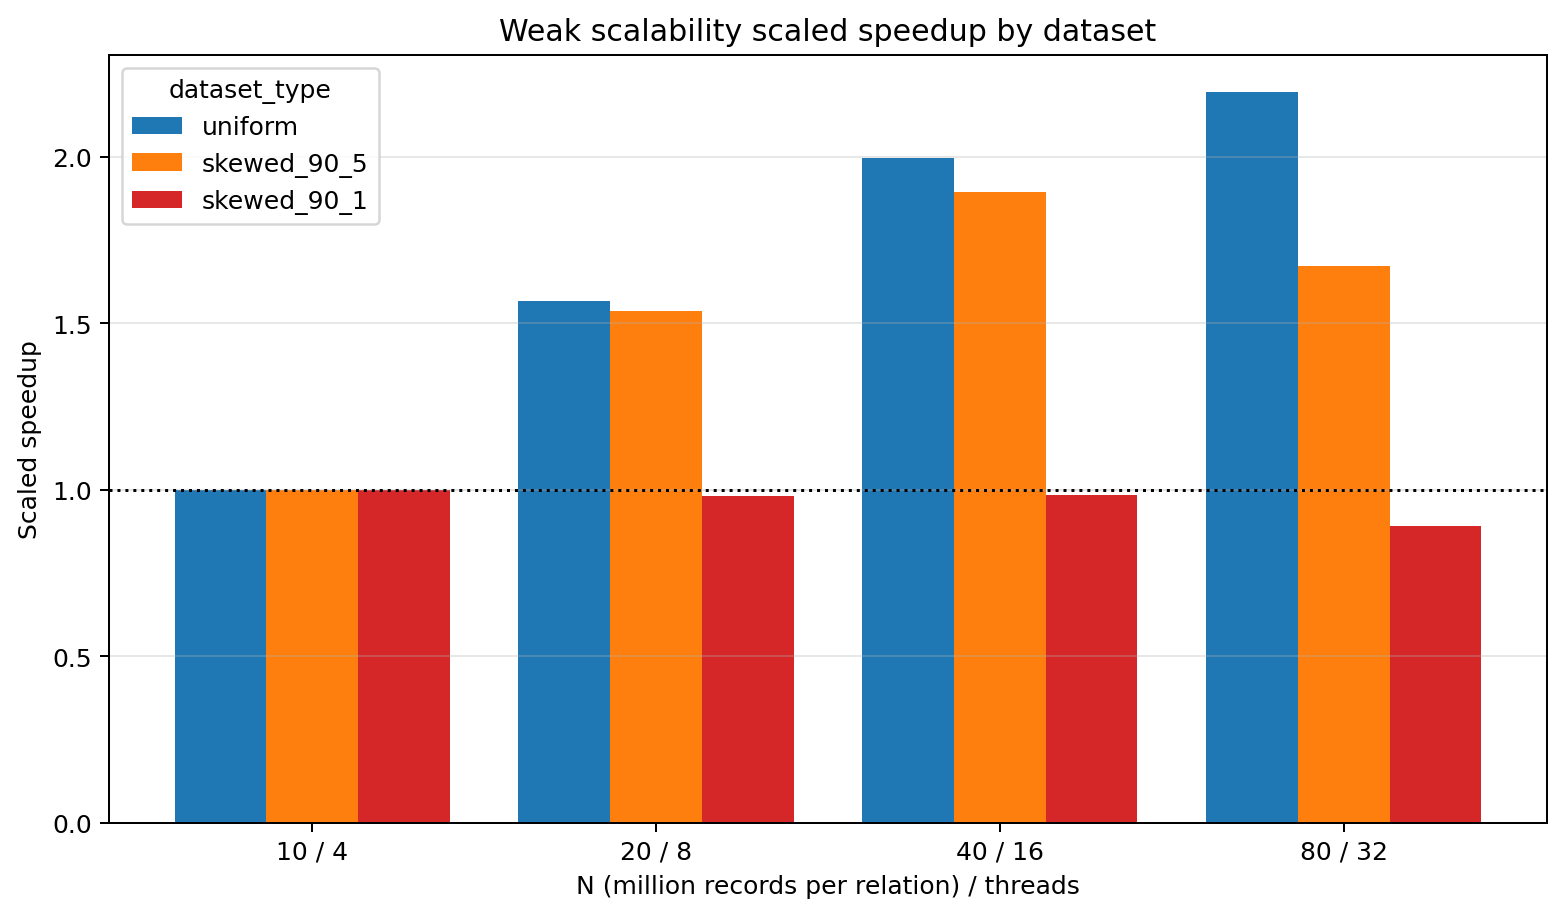
\includegraphics[width=0.48\linewidth]{../img/013_weak_scalability_scaled_speedup_dedicated.png}\hfill
    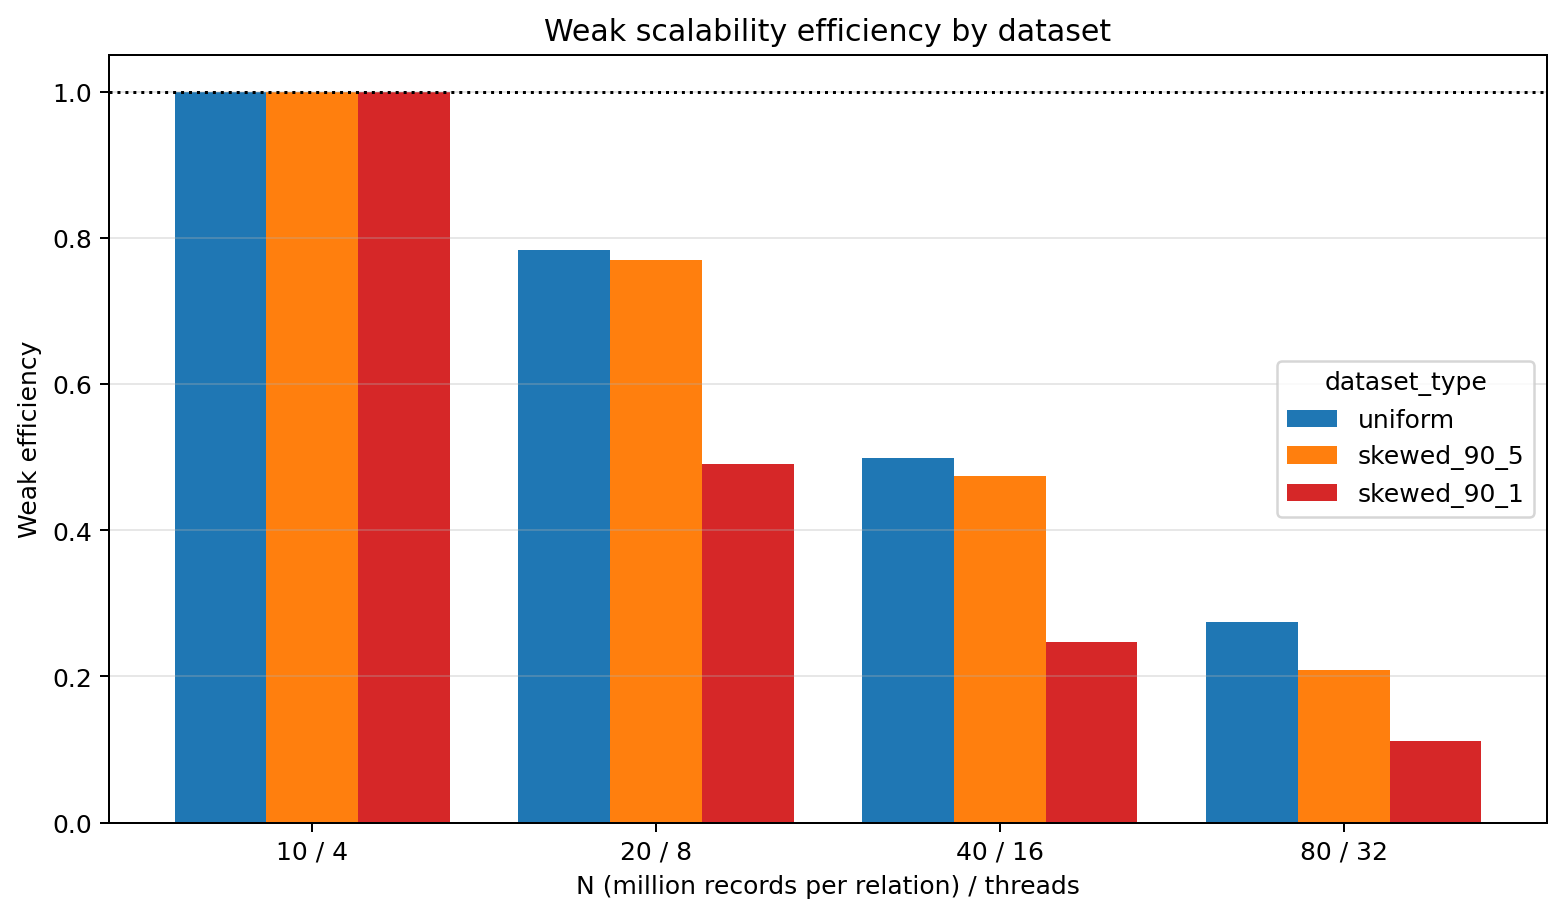
\includegraphics[width=0.48\linewidth]{../img/014_weak_scalability_efficiency_dedicated.png}
    \caption{Weak-scaling scaled speedup and efficiency for uniform and skewed datasets.}
    \label{fig:weak-scaling}
\end{figure}


% Strong scalability
\subsection{Strong scalability}
On the uniform dataset, strong-scaling speedup grows up to \(6.34\times\) at 32 threads and then slightly decreases at 64 threads. The \texttt{skewed\_90\_5} dataset follows the same shape but with a lower plateau, while \texttt{skewed\_90\_1} saturates very early around \(2.9\times\). This confirms that the current granularity is the partition: if one hot partition dominates, adding more threads cannot split that single local join.

\begin{figure}[H]
    \centering
    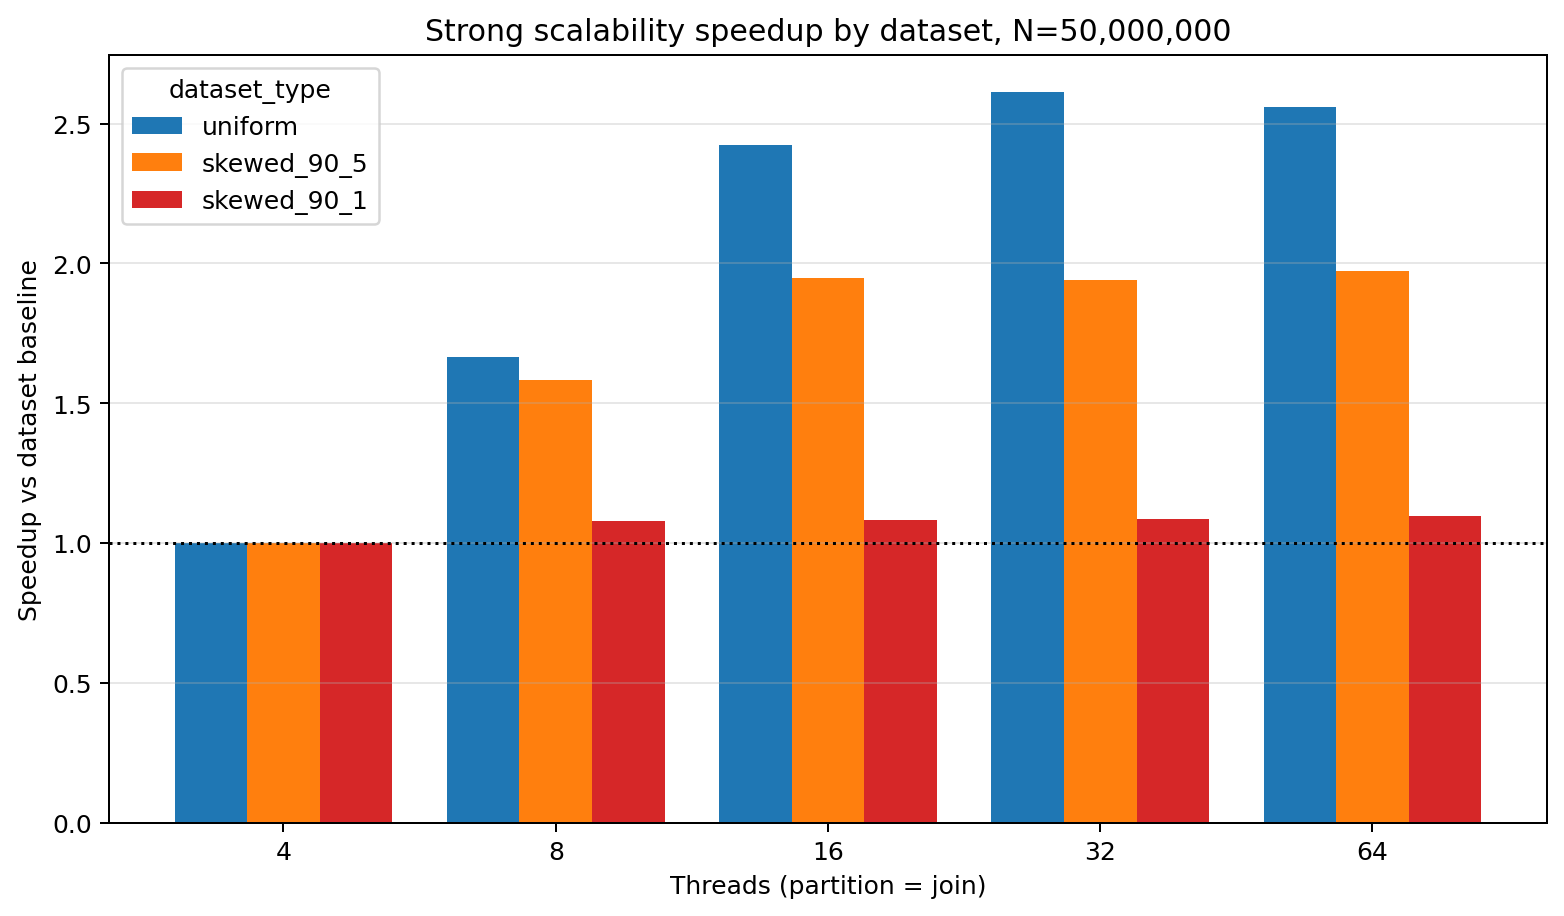
\includegraphics[width=0.48\linewidth]{../img/011_strong_scalability_speedup_dedicated.png}\hfill
    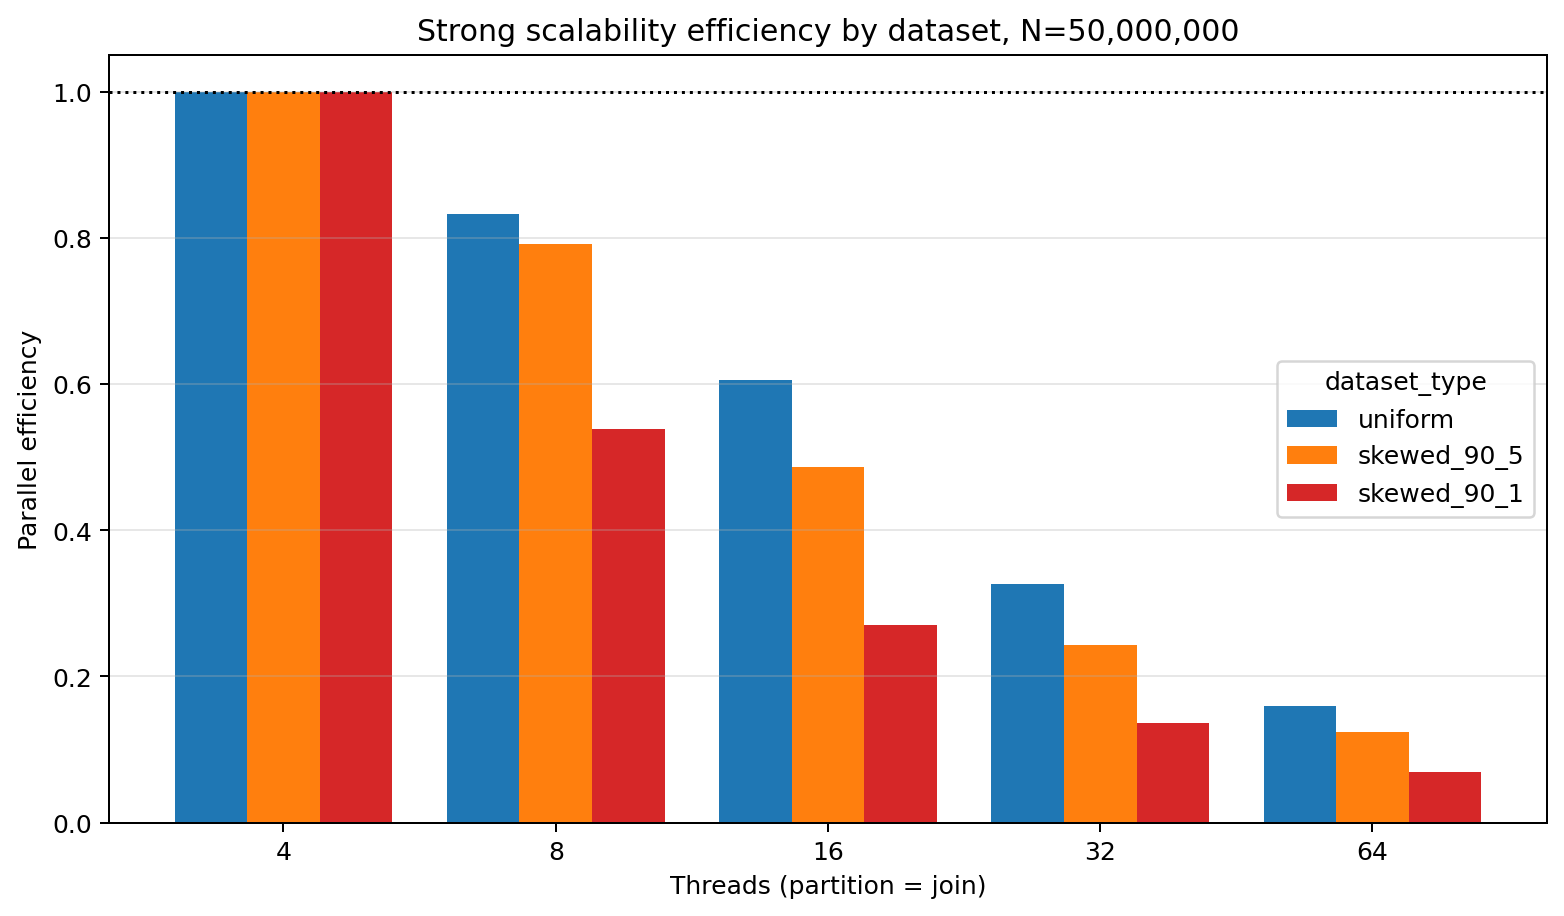
\includegraphics[width=0.48\linewidth]{../img/012_strong_scalability_efficiency_dedicated.png}
    \caption{Strong-scaling speedup and efficiency for the dedicated workload-balanced OpenMP executable.}
    \label{fig:strong-scaling}
\end{figure}


% Correctness validation
\section{Correctness Validation}
Correctness is checked at two levels. For small inputs, each executable can run the naive \(O(N_RN_S)\) verifier and print \texttt{naive\_join\_count}, \texttt{naive\_checksum1} and \texttt{naive\_checksum2}. For benchmark-size inputs, \texttt{checker.cpp} scans the Slurm output files and compares \texttt{join\_count}, \texttt{checksum1} and \texttt{checksum2} for each executable and dataset type. The checker is outside the measured region, and the collected runs match across implementations for the same dataset.


% Conclusions
\section{Conclusions}
The OpenMP implementations preserve the previous algorithm and make the scheduling tradeoffs clearer. On uniform data, loop, task and taskloop variants perform similarly once the join phase is parallelized; tasking does not provide a large advantage because partitions are already well balanced. On skewed data, workload-aware join ordering is the decisive change, especially for \texttt{skewed\_90\_5}. The strongest skew still exposes a limitation of partition-level parallelism: one hot partition cannot be split among multiple threads by the current local join design.

Compared with the best C++ threaded result from Module 2, the best OpenMP result is close but slightly slower in the broad campaign. The main benefit of this module is therefore not a new absolute minimum, but a clearer understanding of which OpenMP constructs are sufficient: guided loop scheduling plus workload-aware dynamic join scheduling is the most robust choice for this implementation.

\end{document}
